\documentclass[a4paper,14pt]{extreport}
	\usepackage[left=1.5cm,right=1.5cm,
	    top=1.5cm,bottom=2cm,bindingoffset=0cm]{geometry}
	\usepackage{scrextend}
	\usepackage[T1,T2A]{fontenc}
	\usepackage[utf8]{inputenc}
	\usepackage[english,russian,ukrainian]{babel}
	\usepackage{tabularx}
	\linespread{1.5}
	\usepackage{amssymb}
	\usepackage{color}
	\usepackage{amsmath}
	\usepackage{mathrsfs}
	\usepackage{listings}
	\usepackage{graphicx}
	\graphicspath{ {./images/} }
	\usepackage{lipsum}
	\usepackage{xcolor}
	\usepackage{multirow}
	%\usepackage[table,xcdraw]{xcolor}
	\usepackage{hyperref}
	\usepackage{tcolorbox}
	\usepackage{tikz}
	\usepackage[framemethod=TikZ]{mdframed}
	\usepackage{wrapfig,boxedminipage,lipsum}
	\mdfdefinestyle{MyFrame}{%
	linecolor=blue,outerlinewidth=2pt,roundcorner=20pt,innertopmargin=\baselineskip,innerbottommargin=\baselineskip,innerrightmargin=20pt,innerleftmargin=20pt,backgroundcolor=gray!50!white}
	 \usepackage{csvsimple}
	 \usepackage{supertabular}
	\usepackage{pdflscape}
	\usepackage{fancyvrb}
	%\usepackage{comment}
	\definecolor{ggreen}{rgb}{0.4,1,0}
	\definecolor{rred}{rgb}{1,0.1,0.1}
	\definecolor{aquamarine}{rgb}{0.5, 1.0, 0.83}
	\definecolor{amber}{rgb}{1.0, 0.75, 0.0}
	\definecolor{babyblue}{rgb}{0.54, 0.81, 0.94}
	\usepackage{array,tabularx}
	\usepackage{colortbl}

	\usepackage{varwidth}
	\tcbuselibrary{skins}
	\usepackage{fancybox}

	\usetikzlibrary{calc}
	\makeatletter
	\newlength{\mylength}
	\xdef\CircleFactor{1.1}
	\setlength\mylength{\dimexpr\f@size pt}
	\newsavebox{\mybox}
	\newcommand*\circled[2][draw=blue]{\savebox\mybox{\vbox{\vphantom{WL1/}#1}}\setlength\mylength{\dimexpr\CircleFactor\dimexpr\ht\mybox+\dp\mybox\relax\relax}\tikzset{mystyle/.style={circle,#1,minimum height={\mylength}}}
	\tikz[baseline=(char.base)]
	\node[mystyle] (char) {#2};}
	\makeatother

	\usepackage{pgfplots}
    \pgfplotsset{compat=1.9}


	\usepackage{float}
	\usepackage{wrapfig}
	\usepackage{framed}
	%for nice Code{
	\lstdefinestyle{customc}{
	  belowcaptionskip=1\baselineskip,
	  breaklines=true,
	  frame=L,
	  xleftmargin=\parindent,
	  language=C,
	  showstringspaces=false,
	  basicstyle=\small\ttfamily,
	  keywordstyle=\bfseries\color{green!40!black},
	  commentstyle=\itshape\color{purple!40!black},
	  identifierstyle=\color{blue},
	  stringstyle=\color{orange},
	}
	\lstset{escapechar=@,style=customc}
	\usepackage{enumitem}
%}

\begin{document}
\newtcbox{\xmybox}[1][red]{on line, arc=7pt,colback=#1!10!white,colframe=#1!50!black, before upper={\rule[-3pt]{0pt}{10pt}},boxrule=1pt, boxsep=0pt,left=6pt,right=6pt,top=2pt,bottom=2pt}
\pagecolor{white}


\begin{landscape}
\begin{enumerate}
	\item Які види взаємодії заряджених частинок в газі ви знаєте?\\
	\texttt{Електронно-атомна взаємодія,Іон-атомні взаємодії,Зіткнення нейтральних частинок, Термічна іонізація, Іонізуюча дія фотонів, Поверхнева іонізація, Утворення негативних іонів, Перезарядка, Електронно-іонна рекомбінація, Рекомбінація на поверхні}

	\item Які умови призводять до пружних та непружних взаємодій?\\
	\texttt{До пружних зіткнень відносяться такі, при 
	яких суми кінетичних енергій частинок до і після зіткнення залишаються незмінними. Поки енергія 
	електрона не досягає значення, що відповідає першому рівню \\
	збудженняатома, можливо лише пружне зіткнення. Після того, як енергія 
	частинки перевищить потенціал збудження або іонізації, ймовірність 
	відповідного процесу різко зростає, а 	потім, при подальшому \\
	збільшенні енергії, знову знижується. Це пояснюється тим, 	що при 	збільшенні енергії зростає швидкість електрона, тобто час взаємодії 	скорочується, отже, менше і ймовірність взаємодії. \\ У разі частих	зіткнень можливе послідовне протікання непружних процесів, 	таких як багаторазова \\ іонізація, ступінчаста  іонізація (іонізація збудженого атома).}

	\item Дайте визначення ефективному перерізу взаємодії.\\
	\texttt{Кількість пружних зіткнень, що відбувається з електроном в 
	середньому на одиниці довжини його шляху, враховується ефективним перерізом пружного зіткнення	$Q_y$. Ефективний переріз обернено пропорційний довжині вільного пробігу $Q_y = \dfrac{1}{\lambda_y}$}

	\item Поясніть залежність перерізів іонізації і перерізів пружного розсіяння від енергій.\\ 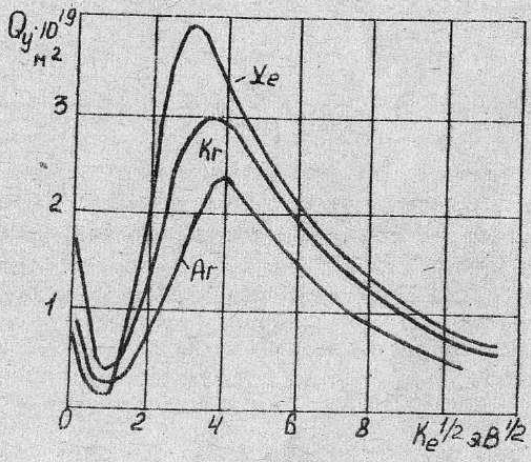
\includegraphics[width=0.3\linewidth]{1.png}\\
	\texttt{Залежність перерізу пружного розсіяння електрона на атомах від його енергії показана на рис. 1.\\ Помітний мінімум при малих швидкостях (енергіях) обумовлений ефектом Рамзауера, пов'язаним із \\взаємодією полів електрона та атома на малих відстанях. При великих швидкостях Qy зменшується\\ внаслідок зниження часу взаємодії між електроном та важкою частинкою.}

	\item Які процеси в газі і на поверхні відбуваються при взаємодії іонів та атомів?\\
	\texttt{}

	\item Розкажіть про особливості термічної іонізації, застосуванні її в техніці.\\
	\texttt{}

	\item Особливості фотонної іонізації.\\
	\texttt{}

	\item Як протікає поверхнева іонізація?\\
	\texttt{}

	\item У чому полягає процес перезарядки?\\
	\texttt{}

	\item  Які види рекомбінації ви знаєте? Опишіть їх.\\
	\texttt{}

	\item  До яких процесів призводить взаємодія лазерного випромінювання з поверхнею твердого тіла і вільними атомами і молекулами?\\
	\texttt{}

	\item  Дайте опис характеру руху заряджених частинок в плазмі.\\
	\texttt{}

	\item  Як оцінюється дрейфовий рух електронів та іонів?\\
	\texttt{}

	\item Розкажіть про основні закономірності дифузійного руху електронів та іонів.\\
	\texttt{}

	\item Дайте визначення плазми. Її особливості, параметри.\\
	\texttt{}

	\item Яка функція розподілу концентрації зарядів по перерізу плазми?\\
	\texttt{}

	\item  Як оцінюється енергетичний стан плазми?\\
	\texttt{}

	\item  Причини виникнення і функція поздовжньої напруженості поля в плазмі\\
	\texttt{}

	\item  Як визначаються електронна та іонна щільності струму в розряді?
	\item  Причини виникнення плазмових коливань в плазма і їх оцінка.
	\item  Які причини призводять до появи таких понять, як провідність плазми та діелектрична проникність?
	\item  Чим зумовлена електропровідність плазами?
	\item  Чим визначається теплопровідність плазми?
	\item  Причини виникнення випромінювання плазми. Види випромінювання.
	\item  Опишіть процес гасіння розряду. Від чого залежить постійна часу деіонізації?
	\item  Як протікає запалювання розряду?
	\item  Що собою уявляє крива Пашена?
	\item  Які методи діагностики плазми ви знаєте?
	\item  Які параметри плазми можна визначити зондовими методами? У чому. їх недоліки?

\end{enumerate}
\end{landscape}













\end{document}